\chapter{General Purpose \texttt{GPU} - \texttt{GP-GPU}}

Le \texttt{GPU} (Graphics Processing Units) e le \texttt{CPU} (Central Processing Units) presentano differenze significative nella loro architettura e nel design, riflettendo le loro finalità di utilizzo orientate rispettivamente al throughput e alla latenza.

\begin{tabular}[b]{c}
  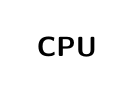
\begin{tikzpicture}[scale=0.4]
    \dram      { 0  ,-2.5}
    \cpucache  { 0  , 0}
    \cpucontrol{ 0  ,4.4}
    \cpualu    { 8.6,4.4}
    \cpualu    {12.8,4.4}
    \cpualu    { 8.6,6.55}
    \cpualu    {12.8,6.55}
    \node[font=\sffamily\bfseries] at (8.45,-3.5) {CPU};
  \end{tikzpicture}\\
  Central Processing Unit (\texttt{CPU})
  \end{tabular}
  \qquad
  \begin{tabular}[b]{c}
  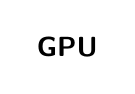
\begin{tikzpicture}[scale=0.4]
    \dram{0,-2.5}
    \foreach \i in {0,...,7}
      \gpucontrol{0,1.1*\i+0.5}
      \gpucache{0,1.1*\i}
      \foreach \j in {1,...,16}
        \gpualu{\j,1.1*\i};
    \node[font=\sffamily\bfseries] at (8.45,-3.5) {GPU};
  \end{tikzpicture}\\
  Graphical Processing Unit (\texttt{GPU})
\end{tabular}

\section{Architettura delle \texttt{CPU}}
Le \texttt{CPU} sono progettate con un'orientamento alla riduzione della latenza:
\begin{itemize}
    \item \textbf{Grandi cache}: Per convertire gli accessi alla memoria a lunga latenza in accessi alla cache a breve latenza.
    \item \textbf{Controllo sofisticato}: Includono la previsione dei branch per ridurre la latenza dei branch e il forwarding dei dati per ridurre la latenza dei dati.
    \item \textbf{\texttt{ALU} potenti}: Unità di elaborazione aritmetica progettate per ridurre la latenza delle operazioni.
\end{itemize}

\section{Architettura delle \texttt{GPU}}
Al contrario, le \texttt{GPU} sono progettate per massimizzare il throughput:
\begin{itemize}
    \item \textbf{Piccole cache}: Ottimizzate per aumentare il throughput della memoria.
    \item \textbf{Controllo semplice}: Non dispongono di previsione dei branch né di forwarding dei dati.
    \item \textbf{\texttt{ALU} efficienti dal punto di vista energetico}: Numerose \texttt{ALU}, caratterizzate da lunghe latenze ma fortemente pipeline per un alto throughput.
    \item \textbf{Necessità di un numero massivo di thread}: Per tollerare le latenze grazie all'alto numero di thread in esecuzione.
\end{itemize}

\section{Differenze nella Gestione della Memoria}
Entrambe le architetture utilizzano la \texttt{DRAM} come memoria principale,
ma si differenziano significativamente nelle loro strategie di gestione della
cache e nel controllo delle unità di elaborazione, riflettendo i loro obiettivi
di progettazione di bassa latenza per le \texttt{CPU} e alto throughput per
le \texttt{GPU}.

\subsection{Comparazione delle Prestazioni tra \texttt{CPU} e \texttt{GPU}}

\paragraph{\texttt{CPU} per Codice Sequenziale}
Le \texttt{CPU} (Central Processing Units) sono ottimizzate per l'esecuzione
di codice sequenziale dove la latenza è un fattore critico. Grazie alla loro
architettura complessa, che include una gestione avanzata della cache e unità
di controllo sofisticate, le \texttt{CPU} possono eseguire codice sequenziale
molto più rapidamente rispetto alle \texttt{GPU}. Questo le rende particolarmente
adatte per applicazioni che richiedono un elevato grado di interattività o tempi
di risposta rapidi, poiché possono essere fino a 10 volte o più veloci delle
\texttt{GPU} nell'esecuzione di codice sequenziale.

\paragraph{\texttt{GPU} per Codice Parallelo}
Al contrario, le \texttt{GPU} (Graphics Processing Units) sono progettate
per massimizzare il throughput, specialmente utile in applicazioni che
beneficiano dell'elaborazione parallela. Con migliaia di core più piccoli,
le \texttt{GPU} gestiscono efficacemente compiti paralleli, distribuendo
il lavoro su molti core per elaborare grandi quantità di dati simultaneamente.
Questo le rende ideali per computazione scientifica, elaborazione di immagini
e applicazioni di machine learning, dove possono superare le \texttt{CPU} di
un fattore di 10 volte o più in termini di velocità.

\paragraph{Scelta dell'Hardware Adatto}
La scelta tra \texttt{CPU} e \texttt{GPU} deve essere fatta in base alla
natura del carico di lavoro. Mentre le \texttt{CPU} sono preferibili per
operazioni che richiedono decisioni rapide e poca parallelizzazione, le
\texttt{GPU} sono la scelta migliore per lavori che possono essere facilmente
suddivisi in compiti più piccoli e gestiti in parallelo. La decisione dovrebbe
quindi basarsi sull'analisi del carico di lavoro specifico e delle esigenze di
prestazione richieste.

\section{Introduzione a \texttt{CUDA C}}
\texttt{CUDA C} è un'estensione del linguaggio di programmazione \texttt{C} che
consente di scrivere codice per le \texttt{GPU} di \texttt{NVIDIA}. Questo
linguaggio permette di sfruttare la potenza di calcolo delle \texttt{GPU} per
eseguire operazioni parallele su grandi quantità di dati. \texttt{CUDA C} è
progettato per essere simile a \texttt{C}, ma include alcune estensioni e
funzionalità specifiche per la programmazione parallela su \texttt{GPU}.



\subsection{Interazione tra \texttt{CPU} e \texttt{GPU}}

In un'applicazione \texttt{CUDA}, la \texttt{CPU} funge da \textbf{host} e
la \texttt{GPU} come \textbf{device}. Il programma inizia la sua esecuzione
sulla \texttt{CPU} con la funzione \texttt{main} e, al richiamo di una
funzione \textbf{kernel}, trasferisce l'esecuzione sulla \texttt{GPU}.
Questo permette di sfruttare l'elaborazione parallela per poi ritornare
alla \texttt{CPU} una volta completate le operazioni sulla \texttt{GPU}.

\subsection{Esecuzione del \texttt{Kernel CUDA}}

Un \textbf{Cuda kernel} è eseguito da una griglia (\textit{array}) di thread.
Tutti i thread in questa griglia eseguono lo stesso codice scritto nel
kernel. È fondamentale identificare ogni thread mediante un indice unico
per garantire che ciascuno esegua il codice in modo appropriatamente ``diverso".

\subsection{Struttura della Grid e Blocchi di Thread}

Le thread non sono aggregate in un unico gruppo all'interno della griglia,
ma sono organizzate in \textbf{blocchi}. Quindi, abbiamo una griglia
composta da blocchi di thread. Questa strutturazione è essenziale
per facilitare la comunicazione e la sincronizzazione delle thread
all'interno dello stesso blocco, grazie alla presenza di una memoria
condivisa. Le thread in blocchi diversi, tuttavia, hanno capacità
limitate di cooperazione diretta, rendendo la memoria condivisa
all'interno dei blocchi uno strumento cruciale per l'efficienza
del parallelismo.


\begin{figure}[H]
  \centering
  \begin{tikzpicture}[font=\small]

    \matrix[label={[anchor=south west, name=gl]north west:Grid}] (OneGrid) [column sep=1mm, row sep=1mm]
    {\pic{block}; & \pic{block}; & \pic{block}; \\
    \pic {block}; & \pic (Ref) {block}; & \pic{block}; \\
    };
    \begin{scope}[on background layer]
    \node[fit=(OneGrid) (gl), inner sep=0pt, fill=green, draw=gray] (Grid) {};
    \end{scope}
    
    
    \matrix[label={[name=ml]Block(1,1)}, below=2cm of Grid] (OneBlock) [column sep=-\pgflinewidth, row sep=\pgflinewidth]
    {\pic{thread}; & \pic{thread}; & \pic{thread}; & \pic{thread}; \\
    \pic{thread}; & \pic{thread}; & \pic{thread}; & \pic{thread}; \\
    \pic{thread}; & \pic{thread}; & \pic{thread}; & \pic{thread}; \\
    };
    \begin{scope}[on background layer]
    \node[fit=(OneBlock) (ml), inner sep=0pt, fill=yellow, draw=gray] (Block) {};
    \end{scope}
    
    \draw[dashed] (RefBl.north west) -- (Block.north west);
    \draw[dashed] (RefBl.north east) -- (Block.north east);
    
    \end{tikzpicture}
\end{figure}

\section{Identificare le Thread in un Kernel \texttt{CUDA}}
La programmazione in \texttt{CUDA} permette di identificare le thread
in uno spazio che può avere fino a tre dimensioni, rappresentate come
\((x, y, z)\). Questo consente agli sviluppatori di adattare l'assegnazione
delle thread alla struttura dei dati che devono essere elaborati.

\subsection{Array Monodimensionale}

Consideriamo il caso di un array di \(128\) elementi. In una struttura
monodimensionale, è naturale assegnare a ogni blocco \(128\) thread,
utilizzando solo la dimensione \(x\) per identificarle. In questo modo,
ogni thread può essere associato direttamente a un elemento dell'array,
e l'indice \texttt{x} del thread corrisponde all'indice dell'elemento
nell'array:

\begin{lstlisting}
    index = threadIdx.x; 
    array[index] = ...; // Operazioni su ogni elemento dell'array
\end{lstlisting}

\subsection{Matrice Bidimensionale}

Per una matrice di dimensioni \(20 \times 20\) \textit{$400$ elementi},
possiamo utilizzare una configurazione bidimensionale per i blocchi
e le thread. Assegnando \(400\) thread per blocco, ogni thread può
essere identificato tramite le coordinate \((x, y)\), permettendo
di mappare direttamente le coordinate della matrice:

\begin{lstlisting}
    row = threadIdx.y;
    col = threadIdx.x; 
    matrix[row][col] = ...; // Operazioni sulla matrice
\end{lstlisting}

\subsection{Strutture Tridimensionali}

Nel caso di strutture tridimensionali, come un cubo, possiamo estendere
ulteriormente questo concetto. I thread e i blocchi possono essere
configurati in tre dimensioni \((x, y, z)\), ognuna corrispondente
a una dimensione del cubo. Questo permette di indirizzare un elemento
specifico dentro un array tridimensionale in modo diretto:

\begin{lstlisting}
    row = threadIdx.y;
    col = threadIdx.x; 
    depth = threadIdx.z;
    cube[row][col][depth] = ...; // Operazioni sul cubo
\end{lstlisting}

\begin{figure}[H]
  \centering 
  \begin{tikzpicture}[line join=round, line cap=round,%
    x={(1 cm,0 cm)}, y={(0 cm,-1cm)}, z={(0.5 cm,0.5 cm)}]
    \foreach\i in {0,1}
    {%
    \cube{(5*\i,0,0)}{4}{yellow}{0}{1}{}{0}
    \foreach\c in {1,0} \foreach\b in {1,0} \foreach\a in {0,1,2} 
    {%
    \cube{(5*\i+1.2*\a-1.2,1.2*\b-0.6,1.2*\c-0.6)}{1}{orange}{1}{0}{$\a,\b,\c$}{0.5+3*\b}
    }
    \cube{(5*\i,0,0)}{4}{none}{1}{0}{Block $\i$}{2}
    }
  \end{tikzpicture}
\end{figure}
\section{Somma tra Vettori in \texttt{CUDA}}
Per esemplificare il concetto di programmazione parallela in \texttt{CUDA},
consideriamo il problema della somma tra due vettori. Questo problema
è particolarmente adatto alla programmazione parallela, poiché ogni
elemento del vettore può essere sommato indipendentemente dagli altri.

\begin{figure}[H]
  \centering
  \begin{tikzpicture}[
    node distance = 5mm and 0mm,
      start chain = A going right,
       box/.style = {rectangle, draw, inner sep=1mm, outer sep=0mm,
                     minimum height=5mm, minimum width=8mm,
                     on chain=A},
        LA/.style = {-{Straight Barb[flex=0]},
                     thick, shorten >=1mm, shorten <=1mm,
                     looseness=1.6}
                            ]
    \node [box, label=left:{$A=$}]  {$A_1$};        % A-1
    \node [box]                     {$A_2$};
    \node [box, densely dashed]     {};
    \node [box]                     {$A_N$};        % A-4
    %
    \node [box, label=left:{$B=$},
           below=of A-1]            {$B_1$};        % A-5
    \node [box]                     {$B_2$};
    \node [box, densely dashed]     {};
    \node [box]                     {$B_N$};        % A-8
    %
    \node [box,right=12mm of $(A-4.east)!0.5!(A-8.east)$]
                                    {$c_1$};  % A-9
    \node [box]                     {$c_2$};
    \node [box, densely dashed]     {};
    \node [box]                     {$c_N$};  % A-12
    %
    \coordinate[left=3mm of A-9.west] (aux);
    \draw[LA]   (A-4) to [out=0, in=180] (aux) -- (A-9);
    \draw[LA]   (A-8) to [out=0, in=180] (aux) -- (A-9);
  \end{tikzpicture}
\end{figure}
\subsection{Versione Sequenziale}
La versione sequenziale di questo algoritmo è molto semplice: basta
scorrere i due vettori e sommare gli elementi corrispondenti.

\begin{lstlisting}
  // Somma tra due vettori
  void vecAdd(float *A, float *B, float *C, int n) {
    for (int i = 0; i < n; i++) {
      C[i] = A[i] + B[i];
    }
  }

  int main()
  {
    // Allocazione e inizializzazione dei vettori
    float *A, *B, *C;
    int n = 1024;
    A = (float *)malloc(n * sizeof(float));
    B = (float *)malloc(n * sizeof(float));
    C = (float *)malloc(n * sizeof(float));
    for (int i = 0; i < n; i++) {
      A[i] = i;
      B[i] = i;
    }
    // Somma tra i vettori
    vecAdd(A, B, C, n);
    // Deallocazione della memoria
    free(A);
    free(B);
    free(C);
    return 0;
  }
\end{lstlisting}

\subsection{Processo di Parallelizzazione in \texttt{CUDA}}

La programmazione in \texttt{CUDA} per l'elaborazione parallela su dispositivi \texttt{GPU} si articola generalmente in tre fasi principali. Queste fasi sono fondamentali per il corretto trasferimento e elaborazione dei dati tra la \texttt{CPU} (host) e la \texttt{GPU} (device).

\subsubsection{Allocazione della Memoria su Device}

Il primo passo in un'applicazione \texttt{CUDA} consiste nell'allocazione della memoria sul device per le variabili necessarie. Per esempio, se abbiamo due array \(A\) e \(B\) che devono essere sommati per ottenere un array \(C\), è necessario allocare la memoria per \(A\), \(B\), e \(C\) sul device:

\begin{lstlisting}
    cudaMalloc(&A, size);
    cudaMalloc(&B, size);
    cudaMalloc(&C, size);
\end{lstlisting}

\subsubsection{Esecuzione del Kernel}

Una volta che la memoria è stata allocata e i dati iniziali sono stati trasferiti al device, il prossimo passo è il lancio del kernel. Il kernel è il codice eseguito parallelamente dai thread della \texttt{GPU}:

\begin{lstlisting}
    dim3 threadsPerBlock(256);
    dim3 numBlocks((N + threadsPerBlock.x - 1) / threadsPerBlock.x);
    addKernel<<<numBlocks, threadsPerBlock>>>(A, B, C);
\end{lstlisting}

Questo esempio mostra un kernel chiamato \texttt{addKernel} che somma due array.

\subsubsection{Copia dei Risultati alla Host Memory}

Dopo l'esecuzione del kernel, l'ultimo passo è copiare il risultato dall'array \(C\) dalla memoria del device alla memoria dell'host. Questo permette all'host di utilizzare i risultati calcolati dalla \texttt{GPU}:

\begin{lstlisting}
    cudaMemcpy(hostC, C, size, cudaMemcpyDeviceToHost);
\end{lstlisting}

\subsection{Versione Parallela in \texttt{CUDA}}

La versione parallela di questo algoritmo utilizza la programmazione parallela
per sfruttare la potenza di calcolo della \texttt{GPU}. Il kernel \texttt{vecAdd}
viene eseguito da un insieme di thread, ognuno dei quali somma un elemento
dei vettori \(A\) e \(B\) per produrre l'elemento corrispondente del vettore \(C\).

\begin{lstlisting}
  __global__ void vecAdd(float *A, float *B, float *C, int n) {
    int i = blockIdx.x * blockDim.x + threadIdx.x;
    if (i < n) {
      C[i] = A[i] + B[i];
    }
  }

  int main()
  {
    // Allocazione e inizializzazione dei vettori
    float *A, *B, *C;
    float *d_A, *d_B, *d_C;
    int n = 1024;
    A = (float *)malloc(n * sizeof(float));
    B = (float *)malloc(n * sizeof(float));
    C = (float *)malloc(n * sizeof(float));
    for (int i = 0; i < n; i++) {
      A[i] = i;
      B[i] = i;
    }
    // Allocazione della memoria sul device
    cudaMalloc(&d_A, n * sizeof(float));
    cudaMalloc(&d_B, n * sizeof(float));
    cudaMalloc(&d_C, n * sizeof(float));
    // Copia dei dati dalla host alla device
    cudaMemcpy(d_A, A, n * sizeof(float), cudaMemcpyHostToDevice);
    cudaMemcpy(d_B, B, n * sizeof(float), cudaMemcpyHostToDevice);
    // Esecuzione del kernel
    vecAdd<<<(n + 255) / 256, 256>>>(d_A, d_B, d_C, n);
    // Copia dei risultati dalla device alla host
    cudaMemcpy(C, d_C, n * sizeof(float), cudaMemcpyDeviceToHost);
    // Deallocazione della memoria
    free(A);
    free(B);
    free(C);
    cudaFree(d_A);
    cudaFree(d_B);
    cudaFree(d_C);
    return 0;
  }
\end{lstlisting}

\subsection{Dimensionamento dei Blocchi e delle Thread}
Quando si esegue un kernel \texttt{CUDA}, è necessario specificare
il numero di blocchi e il numero di thread per blocco. Questi valori
dipendono dalla dimensione del problema e dalla capacità della \texttt{GPU}.
In generale, è consigliabile utilizzare un numero di thread per blocco
che sia un multiplo di \(32\), poiché le \texttt{GPU} di \texttt{NVIDIA}
organizzano i thread in gruppi di \(32\) chiamati \textit{warps}.
\begin{lstlisting}
  dim3 DimGrid((N / 256), 1, 1);
  if (N % 256 != 0) DimGrid.x++;
  dim3 DimBlock(256, 1, 1);

  vecAdd<<<DimGrid, DimBlock>>>(d_A, d_B, d_C, N);
\end{lstlisting}
\subsection{Definizione di Funzioni in \texttt{CUDA}}

Le funzioni in \texttt{CUDA} sono classificate secondo il contesto in
cui possono essere eseguite e da cui possono essere chiamate:

\begin{itemize}
  \item \texttt{\_\_device\_\_ type fun()} - Definisce una funzione che
  può essere chiamata e eseguita solo sul dispositivo (device). Queste
  funzioni sono utilizzate per eseguire calcoli direttamente sulla \texttt{GPU}.
  \item \texttt{\_\_global\_\_ type fun()} - Specifica una funzione che, pur
  essendo definita per il device, viene lanciata dall'host. Questo tipo di
  funzione è comunemente noto come \textit{kernel} e rappresenta il cuore
  dell'esecuzione parallela in \texttt{CUDA}.
  \item \texttt{\_\_host\_\_ type fun()} - Una funzione destinata a essere
  chiamata ed eseguita sull'host, ossia la \texttt{CPU}.
\end{itemize}
In \texttt{CUDA}, è anche possibile definire funzioni che possono
essere eseguite sia sull'host che sul device utilizzando le direttive
\texttt{\_\_host\_\_ \_\_device\_\_}.

\section{Moltiplicazione di Matrici in \texttt{CUDA}}
La moltiplicazione delle matrici può essere espressa come $C = A \times B$,
dove $A$, $B$, e $C$ sono matrici. Ogni elemento della matrice $C$ è il
prodotto scalare di una riga di $A$ e una colonna di $B$. Questo problema
è particolarmente adatto alla programmazione parallela, poiché i calcoli
per ogni elemento di $C$ possono essere eseguiti indipendentemente dagli
altri.

Ogni thread calcola un elemento della matrice $C$ utilizzando la formula
$C_{ij} = \sum_{k=0}^{N-1} A_{ik} \times B_{kj}$, dove $i$ e $j$ sono
gli indici di riga e colonna di $C$, rispettivamente, e $k$ è l'indice
della somma.
\begin{figure}[H]
  \centering
  \begin{tikzpicture}[>=latex]
    \matrix (A) [matrix of math nodes,
                 nodes = {node style ge},
                 left delimiter  = (,
                 right delimiter = )] at (0,0)
    {
      a_{11} & a_{12} & \ldots & a_{1p}  \\
      |[node style sp]| a_{21}
             & |[node style sp]| a_{22}
                      & \ldots
                               & |[node style sp]| a_{2p} \\
      \vdots & \vdots & \ddots & \vdots  \\
      a_{n1} & a_{n2} & \ldots & a_{np}  \\
    };
    \node [draw,below=10pt] at (A.south) 
        { $A$ : \textcolor{red}{$n$ rows} $p$ columns};
    
    \matrix (B) [matrix of math nodes,
                 nodes = {node style ge},
                 left delimiter  = (,
                 right delimiter = )] at (6*\myunit,6*\myunit)
    {
      b_{11} & |[node style sp]| b_{12}
                      & \ldots & b_{1q}  \\
      b_{21} & |[node style sp]| b_{22}
                      & \ldots & b_{2q}  \\
      \vdots & \vdots & \ddots & \vdots  \\
      b_{p1} & |[node style sp]| b_{p2}
                      & \ldots & b_{pq}  \\
    };
    \node [draw,above=10pt] at (B.north) 
        { $B$ : $p$ rows \textcolor{red}{$q$ columns}};
    \matrix (C) [matrix of math nodes,
                 nodes = {node style ge},
                 left delimiter  = (,
                 right delimiter = )] at (6*\myunit,0)
    {
      c_{11} & c_{12} & \ldots & c_{1q} \\
      c_{21} & |[node style sp,red]| c_{22}
                      & \ldots & c_{2q} \\
      \vdots & \vdots & \ddots & \vdots \\
      c_{n1} & c_{n2} & \ldots & c_{nq} \\
    };
    \draw[blue] (A-2-1.north) -- (C-2-2.north);
    \draw[blue] (A-2-1.south) -- (C-2-2.south);
    \draw[blue] (B-1-2.west)  -- (C-2-2.west);
    \draw[blue] (B-1-2.east)  -- (C-2-2.east);
    \draw[<->,red](A-2-1) to[in=180,out=90]
      node[arrow style mul] (x) {$a_{21}\times b_{12}$} (B-1-2);
    \draw[<->,red](A-2-2) to[in=180,out=90]
      node[arrow style mul] (y) {$a_{22}\times b_{22}$} (B-2-2);
    \draw[<->,red](A-2-4) to[in=180,out=90]
      node[arrow style mul] (z) {$a_{2p}\times b_{p2}$} (B-4-2);
    \draw[red,->] (x) to node[arrow style plus] {$+$} (y)%
        to node[arrow style plus] {$+\raisebox{.5ex}{\ldots}+$} (z)
        to (C-2-2.north west);
    
    
    \node [draw,below=10pt] at (C.south) 
        {$ C=A\times B$ : \textcolor{red}{$n$ rows}
                          \textcolor{red}{$q$ columns}};
    
    \end{tikzpicture}
\end{figure}

\subsection{Versione Sequenziale}
La versione sequenziale di questo algoritmo è molto semplice: basta
scorrere le righe di $A$ e le colonne di $B$ per calcolare ogni elemento
di $C$.

\begin{lstlisting}
  // Moltiplicazione tra due matrici
  void matMul(float *A, float *B, float *C, int n, int p, int q) {
    for (int i = 0; i < n; i++) {
      for (int j = 0; j < q; j++) {
        C[i * q + j] = 0;
        for (int k = 0; k < p; k++) {
          C[i * q + j] += A[i * p + k] * B[k * q + j];
        }
      }
    }
  }

  int main()
  {
    // Allocazione e inizializzazione delle matrici
    float *A, *B, *C;
    int n = 1024, p = 512, q = 256;
    A = (float *)malloc(n * p * sizeof(float));
    B = (float *)malloc(p * q * sizeof(float));
    C = (float *)malloc(n * q * sizeof(float));
    for (int i = 0; i < n * p; i++) {
      A[i] = i;
    }
    for (int i = 0; i < p * q; i++) {
      B[i] = i;
    }
    // Moltiplicazione tra le matrici
    matMul(A, B, C, n, p, q);
    // Deallocazione della memoria
    free(A);
    free(B);
    free(C);
    return 0;
  }
\end{lstlisting}

\subsection{Versione Parallela in \texttt{CUDA}}
La programmazione parallela su \texttt{GPU} sfrutta la potenza di
calcolo elevata delle unità di elaborazione grafica per eseguire operazioni
matematiche complesse, come la moltiplicazione di matrici,
in modo significativamente più veloce rispetto ai processori tradizionali.

Per sfruttare al meglio le capacità delle \texttt{GPU}, è cruciale adottare
una rappresentazione efficiente delle matrici. Le matrici \(A\), \(B\) e \(C\)
vengono comunemente rappresentate come array monodimensionali per facilitare
l'accesso e migliorare le prestazioni. Questa rappresentazione, nota come
\textit{row-major order}, organizza le righe della matrice in modo contiguo
nella memoria.

\begin{figure}[H]
    \centering
    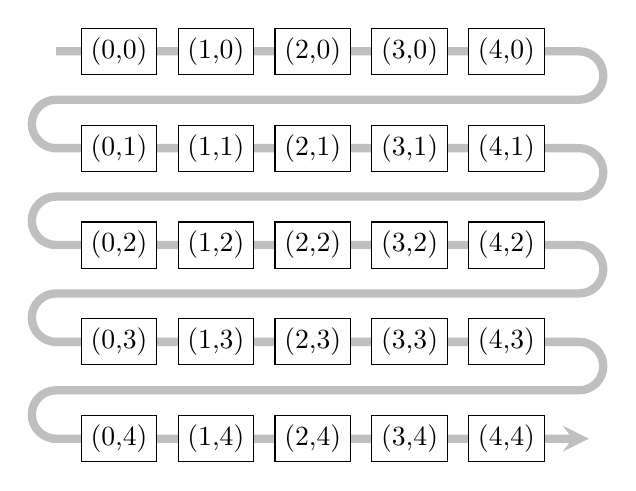
\begin{tikzpicture}[x={(1pt,0)},y={(0,1pt)},scale=0.7]
      \draw[line width=3pt,gray!50,-stealth] (-20,0) 
      \foreach \y in {0,...,3}
      { --  (250,-50*\y) arc(90:-90:12.5)
      --  (-20,-25-50*\y) arc(90:270:12.5)
      -- (-20,-50-50*\y) -- (250, -50-50*\y)
      } --(255,-200);
      \foreach \x in  {0,...,4}
      {\foreach \y in {0,...,4}
       { \node[draw,fill=white] at (12.5+50*\x,-50*\y) (X-\x-\y){(\x,\y)};}
      } 
      \end{tikzpicture}
      \caption{Rappresentazione di una matrice in \textit{row-major order}}
\end{figure}

Nell'ambito della programmazione \texttt{CUDA}, l'accesso agli elementi di
una matrice organizzata secondo il \textit{row-major order} è effettuato
attraverso la seguente formula:
\[
  \texttt{index} = \texttt{row} \times \texttt{width} + \texttt{col}
\]
Questa formula calcola l'indice lineare dell'elemento nella memoria
unidimensionale, dove \texttt{row} rappresenta l'indice della riga,
\texttt{width} la larghezza della matrice, e \texttt{col} l'indice
della colonna.

L'utilizzo del \textit{row-major order} permette un accesso alla memoria
più rapido e prevedibile, essenziale per il parallelismo su \texttt{GPU}.
Gli accessi alla memoria che seguono il pattern naturale della memoria cache
e dei banchi di memoria della \texttt{GPU} riducono i colli di bottiglia
e migliorano il throughput delle operazioni.


\subsection{Gestione dei grid e dei blocchi}
Nella moltiplicazione di matrici tramite \texttt{CUDA}, il dimensionamento
dei blocchi spesso si basa su una tecnica chiamata \textit{tiling}. Questo
approccio permette di ottimizzare l'uso della memoria e migliorare le prestazioni
globali del sistema. Ogni blocco è responsabile del calcolo di un sottoinsieme
della matrice risultante \(C\), e ogni thread all'interno di un blocco calcola
un singolo elemento di \(C\).

Il dimensionamento dei grid e dei blocchi si effettua in modo da dividere
la matrice in ``piastrelle" che possono essere elaborate efficacemente
dai blocchi di thread:

\begin{lstlisting}[language=C]
  // Dimensionamento dei blocchi e dei grid
  dim3 dimGrid(width/TILE_WIDTH, width/TILE_WIDTH, 1);
  dim3 dimBlock(TILE_WIDTH, TILE_WIDTH, 1);
  matMul<<<dimGrid, dimBlock>>>(d_A, d_B, d_C, width);
\end{lstlisting}

Una volta configurati i grid e i blocchi, il kernel \texttt{CUDA} viene
eseguito su ciascun blocco per calcolare i valori corrispondenti nella
matrice \(C\). Il kernel dettagliato è mostrato di seguito:

\begin{lstlisting}[language=C]
  // Definizione del kernel CUDA
  __global__ void matMul(float *A, float *B, float *C, int width) {
    int col = blockIdx.x * blockDim.x + threadIdx.x;
    int row = blockIdx.y * blockDim.y + threadIdx.y;
    float p_val = 0;
    if (row < width && col < width) {
        for (int k = 0; k < width; ++k) {
            p_val += A[row * width + k] * B[k * width + col];
        }
        C[row * width + col] = p_val;
    }
  }
\end{lstlisting}

Questo kernel esegue un ciclo attraverso ogni elemento corrispondente
nelle righe di \(A\) e nelle colonne di \(B\) per accumulare il prodotto
nel valore \(p\_val\), che viene poi assegnato all'elemento corrispondente in \(C\).

\section{Thread \texttt{CUDA}}
Le thread in \texttt{CUDA} sono organizzate in blocchi e griglie, che
forniscono una struttura gerarchica per l'esecuzione parallela. Ogni
thread è identificata da un indice unico all'interno del blocco e della
griglia, che può essere utilizzato per accedere ai dati e coordinare
le operazioni tra le thread.

\section{Modello di Programmazione \texttt{CUDA}}
Il modello di programmazione \texttt{CUDA} consente una scalabilità trasparente attraverso un'assegnazione dinamica dei blocchi di thread e una gestione flessibile delle esecuzioni, adattandosi automaticamente al numero di processori paralleli disponibili.

\subsection{Scalabilità Trasparente nel Modello \texttt{CUDA}}
Nel modello \texttt{CUDA}, l'hardware ha 
la completa libertà di assegnare i blocchi di thread a 
qualsiasi processore in qualsiasi momento, consentendo al kernel 
di scalare su un numero arbitrario di processori paralleli. Questa 
flessibilità è fondamentale per massimizzare l'efficienza di 
esecuzione e le prestazioni del sistema. 

\begin{figure}[H]
  \centering
  \includegraphics[width=0.7\textwidth]{img/transparent_scalability.png}
\end{figure}

\subsection{Dettagli Tecnici di Scheduling e Gestione dei \texttt{SM}}
I blocchi di thread sono organizzati in griglie di blocchi, e ogni blocco 
può essere eseguito in un ordine indipendente rispetto agli altri. 
La granularità dell'assegnazione dei thread ai multiprocessori 
streaming (\texttt{SM}) varia in base alla generazione del processore:
\begin{itemize}
    \item Gli \texttt{SM Fermi} possono gestire fino a $1536$ thread, 
    con configurazioni come $256$ thread per blocco per $6$ blocchi o $512$ thread per blocco per $3$ blocchi.
    \item Gli \texttt{SM Kepler} possono gestire fino a $2048$ thread, 
    con i thread che vengono eseguiti contemporaneamente.
\end{itemize}
Gli \texttt{SM} mantengono e gestiscono gli identificativi di thread 
e blocco, pianificando l'esecuzione dei thread in modo efficiente.

\subsection{Warps come Unità di Scheduling}
All'interno degli \texttt{SM}, ogni blocco viene eseguito come
warps di $32$ thread, che sono le unità di scheduling. Ad esempio,
se a un \texttt{SM} sono assegnati $3$ blocchi e ogni blocco ha
$256$ thread, il numero totale di warps per \texttt{SM} sarà di
$24$, calcolato come \(256/32 = 8\) warps per blocco moltiplicato 
per $3$ blocchi.

\section{Partizione dei Blocchi di Thread e Controllo del Flusso
in \texttt{CUDA}}
Comprendere come i blocchi di thread sono partizionati e gestiti
all'interno del modello di esecuzione di \texttt{CUDA} è fondamentale
per ottimizzare le prestazioni e garantire un comportamento corretto
dell'applicazione.

\subsection{Partizione dei Blocchi di Thread}
I blocchi di thread in \texttt{CUDA} sono partizionati in warp,
con \texttt{ID} di thread consecutivi e crescenti all'interno di
un warp. Questa partizione è consistente tra le esecuzioni, il
che permette ai programmatori di anticipare e pianificare il
comportamento dei thread all'interno dei warp:
\begin{itemize}
    \item Ogni warp inizia con l'\texttt{ID} di thread 0.
    \item I warp sono strutturati in modo che gli \texttt{ID} di
    thread siano sempre consecutivi, migliorando la prevedibilità
    nel controllo del flusso.
\end{itemize}
Tuttavia, i programmatori non dovrebbero fare affidamento su un
ordine specifico tra i warp a causa delle potenziali dipendenze
tra i thread, che necessitano di una sincronizzazione esplicita
utilizzando \texttt{\_\_syncthreads()} per ottenere risultati di esecuzione corretti.

\subsection{Controllo del Flusso in \texttt{CUDA}}
Il controllo del flusso all'interno di \texttt{CUDA} è soggetto a
problemi di divergenza, dove i thread all'interno di un singolo warp
possono seguire percorsi di esecuzione differenti:
\begin{itemize}
    \item La divergenza si verifica quando i thread in un warp seguono
    percorsi di controllo differenti, che vengono poi serializzati,
    potenzialmente degradando le prestazioni.
    \item Un esempio di divergenza: se \texttt{(threadIdx.x > 2)},
    questa condizione crea due percorsi all'interno del primo warp.
    \item Per minimizzare la divergenza, è consigliabile allineare
    le condizioni di ramificazione con i confini dei warp, ad esempio,
    \texttt{if (threadIdx.x / WARP\_SIZE > 2)}.
\end{itemize}

\subsection{Schedulazione e Esecuzione dei Warp}
La schedulazione dei warp è gestita dai Multiprocessori di Streaming
(\texttt{SM}) con zero sovraccarico:
\begin{itemize}
    \item I warp vengono eseguiti in base alla prontezza degli operandi
    e alle politiche di schedulazione prioritarie.
    \item Questo assicura che tutti i thread in un warp eseguano
    la stessa istruzione simultaneamente quando selezionati, ottimizzando il throughput.
\end{itemize}

\subsection{Considerazioni sulla Granularità dei Blocchi per una
Performance Ottimale}
Scegliere la dimensione giusta del blocco è cruciale per la performance,
specialmente in applicazioni come la moltiplicazione di matrici:
\begin{itemize}
    \item Per una configurazione di blocco $8 \times 8$
    (\textit{$64$ thread per blocco}), un \texttt{SM} può supportare
    fino a $24$ blocchi, ma a causa dei vincoli hardware, spesso solo
    $8$ blocchi possono essere attivi contemporaneamente.
    \item Una configurazione di blocco $16 \times 16$
    (\textit{$256$ thread per blocco}) permette a un \texttt{SM}
    di operare vicino alla piena capacità con fino a $6$ blocchi.
    \item Blocchi più grandi, come $32 \times 32$
    (\textit{$1024$ thread per blocco}), possono superare la
    capacità per \texttt{SM} di alcune versioni di \texttt{CUDA}
    e hardware, riducendo l'efficienza.
\end{itemize}

Ciascuna di queste considerazioni gioca un ruolo significativo nel
determinare quanto efficacemente un programma \texttt{CUDA} può operare,
e comprenderle è fondamentale per sfruttare appieno le capacità di \texttt{CUDA}.

\chapter{\texttt{GPU} e memoria}
\section{Panoramica della Memoria in \texttt{CUDA} e Dichiarazione delle Variabili}

\subsection{Accesso alla Memoria nei Thread \texttt{CUDA}}
In \texttt{CUDA}, ogni thread può accedere a diverse tipologie di memoria con tempi di accesso variabili, che influenzano le prestazioni dell'applicazione:
\begin{itemize}
    \item \textbf{Registri per thread:} Ogni thread può leggere e scrivere nei registri specifici per thread con un tempo di accesso molto basso, circa 1 ciclo.
    \item \textbf{Memoria condivisa per blocco:} La memoria condivisa accessibile da tutti i thread di un blocco ha un tempo di accesso di circa 5 cicli.
    \item \textbf{Memoria globale per griglia:} Tutti i thread possono accedere alla memoria globale con un tempo di accesso significativamente più elevato, circa 500 cicli.
    \item \textbf{Memoria costante per griglia:} Accessibile in sola lettura, la memoria costante ha un tempo di accesso di circa 5 cicli se c'è caching.
\end{itemize}

\subsection{Qualificatori delle Variabili in \texttt{CUDA}}
Le variabili in \texttt{CUDA} possono essere qualificate in modo specifico per
definire la loro visibilità e il luogo di memorizzazione. Di seguito è presentata
una tabella che riassume i principali qualificatori delle variabili, la loro
visibilità e i luoghi di memorizzazione.

\begin{table}[H]
\centering
\begin{tabular}{|l|l|l|l|}
\hline
\textbf{Dichiarazione} & \textbf{Memoria} & \textbf{Visibilità} & \textbf{tempo di vita} \\
\hline
\texttt{int LocalVar;} & Registri & Thread & Thread \\
\texttt{\_\_device\_\_ int GlobalVar;} & Globale & Grid & Applicazione \\
\texttt{\_\_device\_\_ \_\_shared\_\_ int SharedVar;} & Condivisa & Blocco & Blocco \\
\texttt{\_\_device\_\_ \_\_constant\_\_ int ConstVar;} & Costante & Grid & Applicazione \\
\hline
\end{tabular}
\caption{Qualificatori delle variabili in \texttt{CUDA} e loro proprietà}
\label{tab:cuda_variable_qualifiers}
\end{table}
\subsubsection{Dove Dichiarare le Variabili?}
\begin{itemize}
    \item Variabili \texttt{global} e \texttt{constant} vanno dichiarate
    all'esterno di qualsiasi funzione per essere accessibili dall'host.
    \item Variabili \texttt{register} (automatiche) e \texttt{shared}
    sono dichiarate all'interno dei kernel.
\end{itemize}

\subsubsection{Esempio}
\begin{lstlisting}
__global__ void MatrixMulKernel(float* d_M, float* d_N, float* d_P, int Width) {
    __shared__ float ds_M[TILE_WIDTH][TILE_WIDTH];
    __shared__ float ds_N[TILE_WIDTH][TILE_WIDTH];
\end{lstlisting}


\section{Strategia di Programmazione Comune in \texttt{CUDA}: Tiling e Blocking}

\subsection{Utilizzo della Memoria Globale e Condivisa}
La memoria globale, situata nella memoria del dispositivo (\texttt{DRAM}), presenta
tempi di accesso lenti. Un metodo efficace per eseguire calcoli sul dispositivo
è quindi quello di usare la tecnica di tiling, che sfrutta la memoria condivisa
più veloce:
\begin{itemize}
    \item \textbf{Partizionamento dei dati:} I dati vengono suddivisi in sottoinsiemi
    che si adattano alla memoria condivisa.
    \item \textbf{Caricamento dei dati:} Ogni blocco di thread carica un sottoinsieme 
    dalla memoria globale alla memoria condivisa, utilizzando più thread per sfruttare 
    il parallelismo a livello di memoria.
    \item \textbf{Computazione sui dati:} I thread eseguono calcoli sui dati nella 
    memoria condivisa. Ogni thread può passare efficientemente più volte su qualsiasi 
    elemento dei dati.
    \item \textbf{Copia dei risultati:} I risultati vengono copiati dalla memoria 
    condivisa alla memoria globale.
\end{itemize}

\subsection{Vantaggi del Tiling e del Blocking}
\begin{itemize}
    \item \textbf{Efficienza:} L'utilizzo di memoria condivisa riduce la latenza di 
    accesso ai dati e aumenta la velocità di esecuzione.
    \item \textbf{Parallelismo a livello di memoria:} Più thread possono caricare e 
    scrivere dati in modo simultaneo, migliorando ulteriormente le prestazioni.
\end{itemize}

\subsection{Considerazioni sul Timing di Accesso dei Thread}
\begin{itemize}
    \item \textbf{Accesso simile:} Il tiling è particolarmente vantaggioso quando i 
    thread hanno tempi di accesso simili, poiché questo permette di massimizzare 
    l'efficienza e minimizzare i conflitti di accesso alla memoria.
    \item \textbf{Accesso diverso:} Se i tempi di accesso dei thread sono molto 
    diversi, il tiling potrebbe non essere efficace e potrebbe portare a una 
    serializzazione indesiderata delle operazioni, riducendo le prestazioni.
\end{itemize}

Queste strategie di programmazione sono cruciali per ottimizzare l'utilizzo delle 
risorse del dispositivo e migliorare le prestazioni generali delle applicazioni 
\texttt{CUDA}.

\section{Moltiplicazione di Matrici in \texttt{CUDA}: Tiling e Blocking}

\subsection{Descrizione dell'Algoritmo}
La moltiplicazione di matrici in \texttt{CUDA} può essere notevolmente
ottimizzata attraverso l'uso del tiling e del blocking. Queste tecniche
sfruttano la memoria condivisa del dispositivo per ridurre il numero di
accessi alla memoria globale, che è più lenta. L'idea di base è suddividere
le matrici in blocchi o ``tiles" più piccoli che possono essere caricati nella
memoria condivisa, permettendo così ai thread di lavorare su porzioni di dati 
più gestibili contemporaneamente.

\subsection{Implementazione in \texttt{CUDA}}
Il kernel \texttt{CUDA} per la moltiplicazione di matrici utilizzando il
tiling segue questi passaggi principali:
\begin{enumerate}
    \item Partizionare le matrici di input in blocchi di dimensioni
    \texttt{TILE\_WIDTH} x \texttt{TILE\_WIDTH}.
    \item Ogni blocco di thread carica un tile di una matrice in memoria condivisa,
    sincronizzandosi con gli altri thread per assicurare che tutti i dati siano
    caricati prima di procedere al calcolo.
    \item Calcolare il prodotto del blocco moltiplicando i corrispondenti tile delle
    due matrici.
    \item Ogni thread accumula il risultato in una variabile locale e, una volta
    completato il calcolo per tutti i tile, scrive il risultato nella memoria globale.
\end{enumerate}

\subsection{Codice \texttt{CUDA} per il Kernel di Moltiplicazione}
Di seguito è riportato un esempio di implementazione di un kernel \texttt{CUDA}
per la moltiplicazione di matrici utilizzando il tiling:

\begin{lstlisting}
__global__ void MatrixMulKernel(float* d_M, float* d_N, float* d_P, int Width) {
    __shared__ float ds_M[TILE_WIDTH][TILE_WIDTH];
    __shared__ float ds_N[TILE_WIDTH][TILE_WIDTH];
    int bx = blockIdx.x; int by = blockIdx.y;
    int tx = threadIdx.x; int ty = threadIdx.y;
    int Row = by * TILE_WIDTH + ty;
    int Col = bx * TILE_WIDTH + tx;
    float Pvalue = 0;
    for (int m = 0; m < Width/TILE_WIDTH; ++m) {
        ds_M[ty][tx] = d_M[Row * Width + (m * TILE_WIDTH + tx)];
        ds_N[ty][tx] = d_N[Col + (m * TILE_WIDTH + ty) * Width];
        __syncthreads();
        for (int k = 0; k < TILE_WIDTH; ++k) {
            Pvalue += ds_M[ty][k] * ds_N[k][tx];
        }
        __syncthreads();
    }
    d_P[Row * Width + Col] = Pvalue;
}
\end{lstlisting}

Questo kernel \texttt{CUDA} esegue la moltiplicazione di matrici utilizzando il tiling
per ottimizzare l'accesso alla memoria e migliorare le prestazioni complessive.

\subsection{Spiegazione del Codice}
\begin{figure}[H]
    \centering
    \includegraphics[width=0.6\textwidth]{img/matrix_mul_tiles.png}
    \caption{Moltiplicazione di matrici con tiling}
\end{figure}
\begin{itemize}
    \item Il kernel carica i tile delle matrici \(M\) e \(N\) in memoria condivisa
    e calcola il prodotto del blocco.
    \item I thread sincronizzano l'accesso alla memoria condivisa per evitare
    conflitti e assicurare che tutti i dati siano disponibili per il calcolo.
    \item Il risultato viene accumulato in una variabile locale e scritto nella
    memoria globale.
\end{itemize}

Questo approccio sfrutta la memoria condivisa per ridurre i tempi di accesso
alla memoria globale e migliorare le prestazioni della moltiplicazione di matrici
su \texttt{CUDA}.

\subsection{Dimensionamento dei Blocchi di Thread e Utilizzo della Memoria Condivisa}
La scelta della dimensione dei blocchi di thread e della larghezza delle tessere (\texttt{TILE\_WIDTH}) ha un impatto significativo sulla performance dei programmi \texttt{CUDA}. 

\begin{itemize}
    \item Un \texttt{TILE\_WIDTH} di $16$ porta a blocchi di $256$
    thread ($16\cdot16$), mentre un \texttt{TILE\_WIDTH} di $32$ comporta
    blocchi di 1024 thread (32x32).
    \item Per una \texttt{TILE\_WIDTH} di $16$, ogni blocco esegue
    $512$ caricamenti di float dalla memoria globale e può eseguire
    $8,192$ operazioni di moltiplicazione/addizione.
    \item Con una \texttt{TILE\_WIDTH} di $32$, il numero di
    operazioni di moltiplicazione/addizione sale a $65536$, per
    un totale di $2048$ caricamenti di float.
\end{itemize}

Queste operazioni di caricamento influenzano direttamente l'utilizzo
della memoria condivisa e la capacità di avere più blocchi attivi
contemporaneamente su un singolo Multiprocessore di Streaming (\texttt{SM}):
\begin{itemize}
    \item Con \texttt{TILE\_WIDTH} = $16$, ogni blocco di thread utilizza
    $2KB$ di memoria condivisa ($2*256*4B$), consentendo potenzialmente
    fino a 8 blocchi di thread attivi contemporaneamente.
    \item Con \texttt{TILE\_WIDTH} = $32$, l'utilizzo di memoria condivisa
    aumenta a $8KB$ per blocco, limitando il numero di blocchi attivi a
    $2$ o $6$ a seconda della configurazione della memoria condivisa e
    della dimensione totale disponibile sull'\texttt{SM}.
\end{itemize}

Utilizzando un tiling di 16x16, si riducono gli accessi alla memoria
globale di un fattore 16, incrementando così efficacemente la larghezza
di banda utilizzabile e il throughput di calcolo.

\subsection{Interrogazione delle Proprietà del Dispositivo}
Per sfruttare al meglio le risorse hardware, è essenziale interrogare
le proprietà del dispositivo \texttt{CUDA} disponibile:
\begin{lstlisting}
int dev_count;
cudaGetDeviceCount(&dev_count);
cudaDeviceProp dev_prop;
for (int i = 0; i < dev_count; i++) {
    cudaGetDeviceProperties(&dev_prop, i);
    // Decisioni basate su dev_prop.maxThreadsPerBlock,dev_prop.sharedMemPerBlock, ...
}
\end{lstlisting}
Questo codice permette di determinare il numero di dispositivi e
le loro specifiche, come il numero massimo di thread per blocco e
la memoria condivisa per blocco, elementi cruciali per configurare
correttamente i kernel.

\subsection{Riepilogo - Struttura Tipica di un Programma \texttt{CUDA}}
Un programma \texttt{CUDA} tipico segue questa struttura:
\begin{enumerate}
    \item Definizione dei kernel e configurazione dei blocchi di thread.
    \item Allocazione e inizializzazione delle strutture di dati.
    \item Trasferimento dei dati dall'host al device.
    \item Esecuzione dei kernel.
    \item Copia dei risultati dal device all'host.
    \item Liberazione delle risorse.
\end{enumerate}
Ripetere questi passi secondo necessità per ottenere il comportamento
desiderato e massimizzare le prestazioni.

\chapter{\texttt{GPU} e considerazioni sulle performance}

\section{Coalescenza della Memoria in \texttt{CUDA}}
La coalescenza della memoria è un concetto chiave per ottimizzare le prestazioni
delle applicazioni \texttt{CUDA}. La coalescenza si riferisce all'accesso
sequenziale e allineato alla memoria da parte dei thread, che consente alla
\texttt{GPU} di combinare le richieste di accesso in un singolo ciclo di
memoria, migliorando così l'efficienza e riducendo i tempi di accesso.

Consideriamo una matrice, rappresentata come un array monodimensionale,
in condizioni normali, l'accesso ai dati da parte dei thread non è
coalescente, poiché i thread accedono a posizioni di memoria non contigue.
Tuttavia, organizzando la matrice in modo che i thread accedano a posizioni
contigue, è possibile ottenere un accesso coalescente, che consente alla
\texttt{GPU} di combinare le richieste di accesso in un singolo ciclo di
memoria.
\begin{figure}[H]
  \centering
  \includegraphics[width=0.8\textwidth]{img/coalescenza.png}
  \caption{Accesso coalescente alla memoria}
\end{figure}
\begin{figure}[H]
  \centering
  \includegraphics[width=0.8\textwidth]{img/non-coalescenza.png}
  \caption{Accesso non coalescente alla memoria}
\end{figure}
\subsection{Coalescenza della memoria}
La coalescenza della memoria si occupa degli accessi alla memoria globale.
A differenza della memoria condivisa, la memoria globale può subire penalità
di prestazioni a causa di accessi non coalescenti. Gli accessi alla memoria
coalescenti riguardano i thread dello stesso warp; l'hardware verifica se gli
accessi alla memoria globale sono eseguiti dai thread dello stesso mezzo warp
e, in tal caso, coalesce gli accessi dei thread in un unico accesso consolidato.

\section{Partizione dinamica delle risorse di esecuzione}
\subsection{Risorse di esecuzione in uno \texttt{SM}}
Le risorse di esecuzione in uno Streaming Multiprocessor (\texttt{SM}) includono
registri, memoria condivisa e slot per blocchi di thread. Analizziamo un
dispositivo con un massimo di $1536$ thread per \texttt{SM}:
\begin{itemize}
  \item Con blocchi da $512$ thread, è possibile ospitare 3 blocchi per \texttt{SM},
  una configurazione ottimale.
  \item Con blocchi da $128$ thread, si teorizzano $12$ blocchi per \texttt{SM}, ma questo
  supera le capacità e si limita a $8$ blocchi da $128$ thread ciascuno, totalizzando
  $1024$ thread, sotto-utilizzando così le capacità dello \texttt{SM}.
\end{itemize}

\subsection{Gestione dei registri per \texttt{SM}}
Considerando uno \texttt{SM} con $16384$ registri disponibili:
\begin{itemize}
  \item Se un kernel istanzia 10 variabili ($32$ bit) per thread:
  \begin{itemize}
    \item Con blocchi da $256$ thread, si necessitano 2560 registri per blocco.
    \item Con un rapporto di $1536$ thread per \texttt{SM} suddivisi in blocchi da
    $256$ thread, si possono ospitare $6$ blocchi, che utilizzano 15360 registri in
    totale, una configurazione accettabile.
    \item Aggiungere anche solo un blocco ulteriore per \texttt{SM} comporterebbe
    il superamento del limite di registri disponibili, richiedendo una riduzione
    nel numero di blocchi.
  \end{itemize}
  \item Aggiungendo due variabili per kernel ($12$ variabili in totale per thread):
  \begin{itemize}
    \item Ogni blocco da $256$ thread richiederebbe 3072 registri.
    \item Sei blocchi da $3072$ registri ciascuno comportano un totale di 18432
    registri, superando il limite. La soluzione comporta una riduzione del
    numero di blocchi a 5, rientrando così nei $15360$ registri disponibili,
    ma riducendo il numero di thread attivi per \texttt{SM} a $1280$ anziché $1536$, a
    causa dell'aumento del numero di variabili.
  \end{itemize}
\end{itemize}

\section{Parallelizzazione dei task per il trasferimento dati}
Quando si schedula un kernel, è possibile definire un grafo di dipendenza tra
le esecuzioni dei kernel e i trasferimenti di memoria. Per esempio, il kernel
A non può eseguire
fino a quando non sono completati i trasferimenti di dati A e B, ma può iniziare
mentre il trasferimento C è ancora in corso.

\texttt{CUDA} offre la possibilità di eseguire operazioni di trasferimento dati
e computazione in modo asincrono attraverso l'uso degli stream. Gli stream
permettono di eseguire trasferimenti di dati e kernel in parallelo, migliorando
l'utilizzo delle risorse e riducendo i tempi di attesa.
\section{Device Overlap}

Nel contesto della programmazione \texttt{CUDA}, il \texttt{deviceOverlap}
rappresenta una funzionalità importante per aumentare l'efficienza e
la velocità di esecuzione dei programmi. Questa funzione permette ai
dispositivi \texttt{CUDA} di eseguire simultaneamente un kernel
e una operazione di copia di memoria tra il dispositivo e l'host.

\section*{Verifica del Supporto a \texttt{deviceOverlap}}
Per determinare se un dispositivo \texttt{CUDA} supporta il
\texttt{deviceOverlap},
è possibile utilizzare il seguente codice:

\begin{lstlisting}
int dev_count; 
cudaDeviceProp prop;
cudaGetDeviceCount(&dev_count);
for (int i = 0; i < dev_count; i++) {
    cudaGetDeviceProperties(&prop, i);
    if (prop.deviceOverlap) {
        // Il dispositivo supporta deviceOverlap
    }
}
\end{lstlisting}

Questo frammento di codice prima interroga il numero totale di dispositivi
\texttt{CUDA} disponibili. Successivamente, per ogni dispositivo, acquisisce
e analizza le sue proprietà attraverso \texttt{cudaGetDeviceProperties} per
verificare la presenza della caratteristica \texttt{deviceOverlap}.

\section*{Utilizzo del Timing Sovrapposto (Pipelined)}
Una tecnica efficace per sfruttare al meglio il \texttt{deviceOverlap}
consiste nel dividere i vettori di grandi dimensioni in segmenti più piccoli
e gestire il trasferimento e il calcolo di questi segmenti in maniera
sovrapposta. Questo approccio, noto come \textit{pipelined timing},
permette di ridurre i tempi morti in cui il dispositivo potrebbe altrimenti
rimanere inattivo, ottimizzando così sia le operazioni di trasferimento che
quelle di calcolo.

\subsection{Stram di \texttt{CUDA}}
Il parallelismo di task in \texttt{CUDA} è realizzato mediante divers
 \texttt{streams}. Le operazioni inserite in \texttt{streams} differenti
 possono essere eseguite in parallelo. Questo è particolarmente utile per
 sovrapporre la copia di memoria e l'esecuzione di kernel, migliorando
 l'efficienza complessiva del programma.

Le richieste di dispositivo effettuate dal codice host sono inserite
in una coda, che viene letta ed elaborata in modo asincrono dal driver
e dal dispositivo. Il driver assicura che i comandi nella coda siano
processati in sequenza, garantendo che le copie di memoria siano
completate prima del lancio dei kernel, tra gli altri.

Per permettere la copia e l'esecuzione di kernel in modo concorrente, è
necessario utilizzare più code, denominate \texttt{streams}. Gli ``eventi"
\texttt{CUDA} permettono al thread host di interrogare e sincronizzarsi
con le code individuali.

\section*{Codice Host Multi-Stream Semplice}
Di seguito è presentato un esempio di codice host che utilizza due
\texttt{streams} per gestire le operazioni in modo parallelo:

\begin{lstlisting}[language=C]
cudaStream_t stream0, stream1;
cudaStreamCreate(&stream0);
cudaStreamCreate(&stream1);

float *d_A0, *d_B0, *d_C0; // memoria del dispositivo per stream 0
float *d_A1, *d_B1, *d_C1; // memoria del dispositivo per stream 1

// Allocazione di cudaMalloc per d_A0, d_B0, d_C0, d_A1, d_B1, d_C1

for (int i = 0; i < n; i += SegSize * 2) {
    cudaMemCpyAsync(d_A0, h_A + i, SegSize * sizeof(float), ..., stream0);
    cudaMemCpyAsync(d_B0, h_B + i, SegSize * sizeof(float), ..., stream0);
    vecAdd<<<SegSize / 256, 256, 0, stream0>>>(d_A0, d_B0, ...);
    cudaMemCpyAsync(d_C0, h_C + i, SegSize * sizeof(float), ..., stream0);

    cudaMemCpyAsync(d_A1, h_A + i + SegSize, SegSize * sizeof(float), ..., stream1);
    cudaMemCpyAsync(d_B1, h_B + i + SegSize, SegSize * sizeof(float), ..., stream1);
    vecAdd<<<SegSize / 256, 256, 0, stream1>>>(d_A1, d_B1, ...);
    cudaMemCpyAsync(d_C1, h_C + i + SegSize, SegSize * sizeof(float), ..., stream1);
}
\end{lstlisting}

Il problema di questo codice è che non avviene in trasferimento dei dati
nel momento in cui il kernel esegue la somma vettoriale. Questo problema
può essere risolto riorganizzando il codice in modo che i trasferimenti
di dati avvengano in modo corretto:
\begin{lstlisting}[language=C]
for (int i = 0; i < n; i += SegSize * 2) {
    cudaMemCpyAsync(d_A0, h_A + i, SegSize * sizeof(float), ..., stream0);
    cudaMemCpyAsync(d_A1, h_A + i + SegSize, SegSize * sizeof(float), ..., stream1);
    cudaMemCpyAsync(d_B0, h_B + i, SegSize * sizeof(float), ..., stream0);
    cudaMemCpyAsync(d_B1, h_B + i + SegSize, SegSize * sizeof(float), ..., stream1);

    vecAdd<<<SegSize / 256, 256, 0, stream0>>>(d_A0, d_B0, ...);
    vecAdd<<<SegSize / 256, 256, 0, stream1>>>(d_A1, d_B1, ...);

    cudaMemCpyAsync(d_C0, h_C + i, SegSize * sizeof(float), ..., stream0);
    cudaMemCpyAsync(d_C1, h_C + i + SegSize, SegSize * sizeof(float), ..., stream1);
}
\end{lstlisting}

\subsection{Concorrenza in Fermi e Precedenti}
Le architetture \texttt{GPU} di \texttt{NVIDIA} precedenti a Kepler, come Fermi,
supportavano una concorrenza a $16$ vie. Questo significava che fino a
$16$ griglie potevano essere eseguite contemporaneamente. Tuttavia, le
\texttt{CUDA streams} venivano multiplexate in una singola coda hardware
per l'esecuzione, limitando la concorrenza a livello di stream.

\subsection{Hyper Queue in Kepler}
Con l'introduzione di Kepler, \texttt{NVIDIA} ha implementato Hyper Queue,
che fornisce multiple code reali per ciascun motore, permettendo una maggiore
concorrenza. Questo approccio consente ad alcune stream di fare progressi
per un motore mentre altre possono essere bloccate, migliorando l'efficienza
e la scalabilità.

\subsection{Miglioramento della Concorrenza con Kepler}
Kepler ha significativamente migliorato la concorrenza rispetto a Fermi,
consentendo una concorrenza a $32$ vie. Ogni stream ha una propria coda
di lavoro dedicata, che elimina le dipendenze inter-stream e consente
la concorrenza a livello di intero stream, migliorando così le
prestazioni generali:

\begin{itemize}
    \item \textbf{Concorrenza $32$-vie:} Ogni \texttt{GPU} Kepler può gestire
    fino a $32$ stream contemporaneamente.
    \item \textbf{Code di lavoro multiple:} Una coda di lavoro per ogni stream.
    \item \textbf{Nessuna dipendenza inter-stream:} Ogni stream opera
    indipendentemente dagli altri, permettendo una migliore scalabilità
    e efficienza.
\end{itemize}
\section{Introduzione al Prefix Scan}
L'operazione di \textbf{Prefix Scan}, prende in input:
\begin{itemize}
  \item Un operatore binario associativo $\oplus$.
  \item Un array di $N$ elementi $[x_0, x_1, \dots, x_{N-1}]$.
\end{itemize}
Essa restituisce un array trasformato che può essere:
\begin{itemize}
  \item \textbf{Inclusivo:} $[x_0, (x_0 \oplus x_1), \dots,
  (x_0 \oplus x_1 \oplus \dots \oplus x_{N-1})]$.
  \item \textbf{Esclusivo:} $[0, x_0, (x_0 \oplus x_1), \dots,
  (x_0 \oplus x_1 \oplus \dots \oplus x_{N-2})]$.
\end{itemize}

\subsubsection{Esempio}
Per $\oplus$ come addizione (somma prefissa):
\begin{itemize}
  \item \textbf{Inclusivo:} Da $[3, 1, 7, 4, 6]$ a $[3, 4, 11, 15, 21]$.
  \item \textbf{Esclusivo:} Da $[3, 1, 7, 4, 6]$ a $[0, 3, 4, 11, 15]$.
\end{itemize}
\begin{figure}[H]
  \centering
  \includegraphics[width=0.7\textwidth]{img/scan_1.png}
  \caption{Esempio di Prefix Scan}
\end{figure}
\subsubsection{Conversione tra Scansioni Inclusive ed Esclusive}
\begin{itemize}
  \item Da esclusiva a inclusiva:
  \begin{itemize}
    \item Spostare l'array risultante di un elemento a sinistra.
    \item Inserire alla fine la somma dell'ultimo elemento della
    scansione e l'ultimo elemento dell'array di input.
  \end{itemize}
  \item Da inclusiva a esclusiva:
  \begin{itemize}
    \item Spostare l'array risultante di un elemento a destra.
    \item Inserire l'identità all'inizio.
  \end{itemize}
\end{itemize}

\subsection{Usi del Prefix Scan}
Il Prefix Scan è una primitiva chiave in molti algoritmi paralleli
per convertire calcoli seriali in paralleli, utilizzato in:
\begin{itemize}
  \item Ordinamento (counting sort/radix sort)
  \item Istogramma
  \item Inserimento in coda di massa
  \item Compattazione di flusso/Partizione
  \item Moltiplicazione di matrici sparse
  \item Costruzione di strutture dati in parallelo
  \item e altro...
\end{itemize}

\subsection{Implementazione Sequenziale}
\textbf{Inclusivo:}
\begin{lstlisting}
Out[0] = In[0];
for (int i = 1; i < N; ++i) {
  Out[i] = Out[i-1] + In[i];
}
\end{lstlisting}

\textbf{Esclusivo:}
\begin{lstlisting}
Out[0] = 0;
for (int i = 1; i < N; ++i) {
  Out[i] = Out[i-1] + In[i-1];
}
\end{lstlisting}
\textbf{Nota:} Sono necessarie $N$ addizioni per $N$ elementi,
con una complessità di $O(n)$.

\subsection{Prefix Scan Parallelo}

Di seguito è riportato l'algoritmo per un'implementazione parallela naive del
Prefix Scan, usando un approccio iterativo che aumenta progressivamente la
distanza tra gli elementi combinati ad ogni step.

\begin{algorithm}[H]
\caption{Naive Parallel Prefix Scan}
\label{alg:parallel_prefix_scan}
  \For{$int \texttt{ level} = 0$; $level < \log_2(N)$; $\texttt{++level}$}{
    \ForPar{$\forall i \in N$}{
      \texttt{offset} = $2^{\texttt{level}}$\\
    }
    \If{$i \geq \texttt{offset}$}{
      $X[i] = X[i - \texttt{offset}] + X[i]$\\
    }
    }
\end{algorithm}

La complessità parallela, \textit{span}, di questo algoritmo è $O(\log(N))$, 
mentre la complessità di lavoro è $O(n \cdot \log(n))$, dove $n$ è il numero di
elementi da scansionare, poiché ogni elemento deve essere combinato con tutti
gli altri.

\section{Prefix scan per l'efficienza di lavoro}
L'algoritmo consiste in due fasi principali:
\begin{itemize}
  \item \textit{up-sweep}: calcola la somma prefissa per ogni potenza di $2$.
  \item \textit{down-sweep}: calcola la somma prefissa finale.
\end{itemize}
\begin{figure}[H]
  \centering
  \includegraphics[width=0.7\textwidth]{img/scan_2_fase1.png}
  \caption{Fase 1: Up-Sweep}
\end{figure}
\begin{figure}[H]
  \centering
  \includegraphics[width=0.7\textwidth]{img/scan_2_fase2.png}
  \caption{Fase 2: Down-Sweep}
\end{figure}

Di seguito è riportato il codice per l'implementazione parallela del Prefix Scan
con efficienza di lavoro:

\begin{algorithm}[H]
\caption{Efficient Parallel Prefix Scan}
\label{alg:efficient_parallel_prefix_scan}
\For{$\texttt{level} = 0$; $\texttt{level} < \log_2(N)$; $\texttt{++level}$}{
  \texttt{step} = $2^{\texttt{level}}$\\
  \ForPar{$\forall i \mid i \mod (\texttt{step} \cdot 2) = 0$}{
    \texttt{valueRight} = $(i + 1) \cdot (step \cdot 2) - 1$\\
    \texttt{valueLeft} = \texttt{valueRight} - \texttt{step}\\
    $X[\texttt{valueRight}] = X[\texttt{valueRight}] + X[\texttt{valueLeft}]$\\
  }
}
\end{algorithm}

In questo modo si riduce la complessità di lavoro a $O(n)$, mantenendo
una complessità parallela di $O(\log(n))$.